% !TEX program = pdflatex
\documentclass[12pt,a4paper]{article}

% =========================================================
% Encodage & langue
% =========================================================
\usepackage{needspace}
\usepackage{booktabs}
\usepackage{tabularx}
\usepackage{tcolorbox}
\tcbuselibrary{breakable}

\newcommand{\NewMajorPart}{\clearpage}
\newcommand{\SubNeeds}[1]{\Needspace{#1\baselineskip}}

\newcommand{\roundedimg}[2][width=\textwidth]{%
  \sbox0{\includegraphics[#1]{#2}}%
  \begin{tikzpicture}
    \clip[rounded corners=10pt] (0,0) rectangle (\wd0,\ht0);
    \node[anchor=south west, inner sep=0pt] at (0,0) {\usebox0};
  \end{tikzpicture}%
}

\usepackage[T1]{fontenc}
\usepackage[utf8]{inputenc}
\usepackage[french]{babel}
\usepackage{longtable}
\usepackage{float}

% =========================================================
% Index
% =========================================================
\usepackage{makeidx}
\makeindex

% =========================================================
% Police
% =========================================================
\usepackage{helvet}
\renewcommand{\familydefault}{\sfdefault}

% =========================================================
% Paragraphes
% =========================================================
\setlength{\parindent}{1.25em}
\setlength{\parskip}{0pt}

% =========================================================
% Mise en page
% =========================================================
\usepackage{geometry}
\geometry{margin=2.5cm, headheight=14.5pt}
\usepackage{setspace}
\onehalfspacing

% =========================================================
% Listes
% =========================================================
\usepackage{enumitem}

\newlist{sq}{itemize}{1}
\setlist[sq]{%
  label=\rule{0.9ex}{0.9ex},
  leftmargin=3.2em,
  labelsep=0.35em,
  itemsep=0.1em,
  parsep=0pt,
  topsep=0.12em,
  partopsep=0pt
}

\newlist{num}{enumerate}{1}
\setlist[num]{%
  label=\textbf{[\arabic*]},
  leftmargin=3.2em,
  labelsep=0.35em,
  itemsep=0.1em,
  parsep=0pt,
  topsep=0.12em,
  partopsep=0pt
}

\setlist[itemize]{leftmargin=2.2em, itemsep=0.2em, topsep=0.2em}
\setlist[enumerate]{leftmargin=2.2em, itemsep=0.2em, topsep=0.2em}

% =========================================================
% Graphiques & en-têtes
% =========================================================
\usepackage{graphicx}
\usepackage{tikz}
\usepackage{xcolor}
\usepackage{colortbl}
\usepackage{fancyhdr}
\usepackage[hidelinks]{hyperref}
\usepackage{tcolorbox}
\tcbuselibrary{skins}
\newtcolorbox{promptbox}{
  colback=teal!5!white,
  colframe=teal,
  boxrule=0.6pt,
  arc=6pt,
  left=10pt, right=10pt, top=6pt, bottom=6pt,
  title={\textbf{Prompt IA}},
  fonttitle=\small\bfseries,
  coltitle=white,
  attach boxed title to top left={yshift=-2mm, xshift=6pt},
  boxed title style={colback=teal, colframe=teal},
  breakable,
}
\usepackage{caption}
\captionsetup{font=small, labelfont=bf}
\usepackage{listings}
\usepackage{amssymb}
\usepackage{multicol}
\usepackage{tocloft}
\setlength{\cftbeforesecskip}{0.6em}
\setlength{\cftbeforesubsecskip}{0.25em}
\newcommand{\cmark}{\textcolor{green!55!black}{\boldmath$\checkmark$}}
\newcommand{\xmark}{\textcolor{red!70!black}{\boldmath$\times$}}

% =========================================================
% Styles de page
% =========================================================
\pagestyle{fancy}
\fancyhf{}
\lhead{\textbf{MEDISCAN AI}}
\rhead{\textbf{Rapport de Projet}}
\cfoot{\thepage}

\fancypagestyle{firstpage}{
  \fancyhf{}
  \cfoot{\thepage}
  \renewcommand{\headrulewidth}{0pt}
  \renewcommand{\footrulewidth}{0pt}
}

% =========================================================
% Macro
% =========================================================
\newcommand{\IntroPartie}[1]{%
\vspace{0.2cm}
\begin{center}
\textit{#1}
\end{center}
\vspace{0.3cm}
}

% =========================================================
% Titre
% =========================================================
\title{Rapport de Projet --- \textbf{MEDISCAN AI}\\[0.4em]
\large Plateforme de recherche multimodale d'images médicales par le contenu (\textbf{CBIR})}
\author{L3X1 --- Université Paris Cité}
\date{}

% =========================================================
\begin{document}
% =========================================================

% =========================================================
% PAGE DE GARDE
% =========================================================
\maketitle
\thispagestyle{firstpage}

\vspace{0.3cm}
\begin{center}
  
\includegraphics[width=0.5\textwidth]{assets/Logo.png}
\end{center}

\vspace{0.5cm}

\begin{center}
\textit{
Le présent document est le \textbf{rapport de projet} de \textbf{MEDISCAN AI},
prototype académique non clinique de recherche d'images médicales par le contenu.
Il couvre l'ensemble des travaux de l'équipe L3X1 : besoins, conception,
implémentation, tests et déploiement.
}
\end{center}

\vspace{0.8cm}

\section*{Informations document}
{\setlength{\parindent}{0pt}
\begin{tabularx}{\textwidth}{@{}lX@{}}
\textbf{Version :}         & v1.0 \\
\textbf{Référence :}       & Rapport de Projet MEDISCAN AI v1.0 \\
\textbf{Confidentialité :} & Interne projet (usage universitaire) \\
\textbf{Encadrant :}       & Camille Kurtz \\
\textbf{Équipe :}          & L3X1 (Taskin Ozan, Rayane Taouache, Ales Ferhani, Maxime Huang) \\
\end{tabularx}
}

% =========================================================
% ÉQUIPE
% =========================================================
\newpage
\section*{Équipe projet}
\addcontentsline{toc}{section}{Équipe projet}

\vspace{1.0cm}
L'équipe \textbf{L3X1} est composée de quatre étudiants de l'Université Paris Cité.
Chaque membre a contribué à plusieurs pôles en fonction de ses compétences.

\vspace{1.5cm}

\begin{center}
\begin{tabular}{cccc}
  \begin{tikzpicture}
    \clip (0,0) circle (1.2cm);
    \node at (0,0) {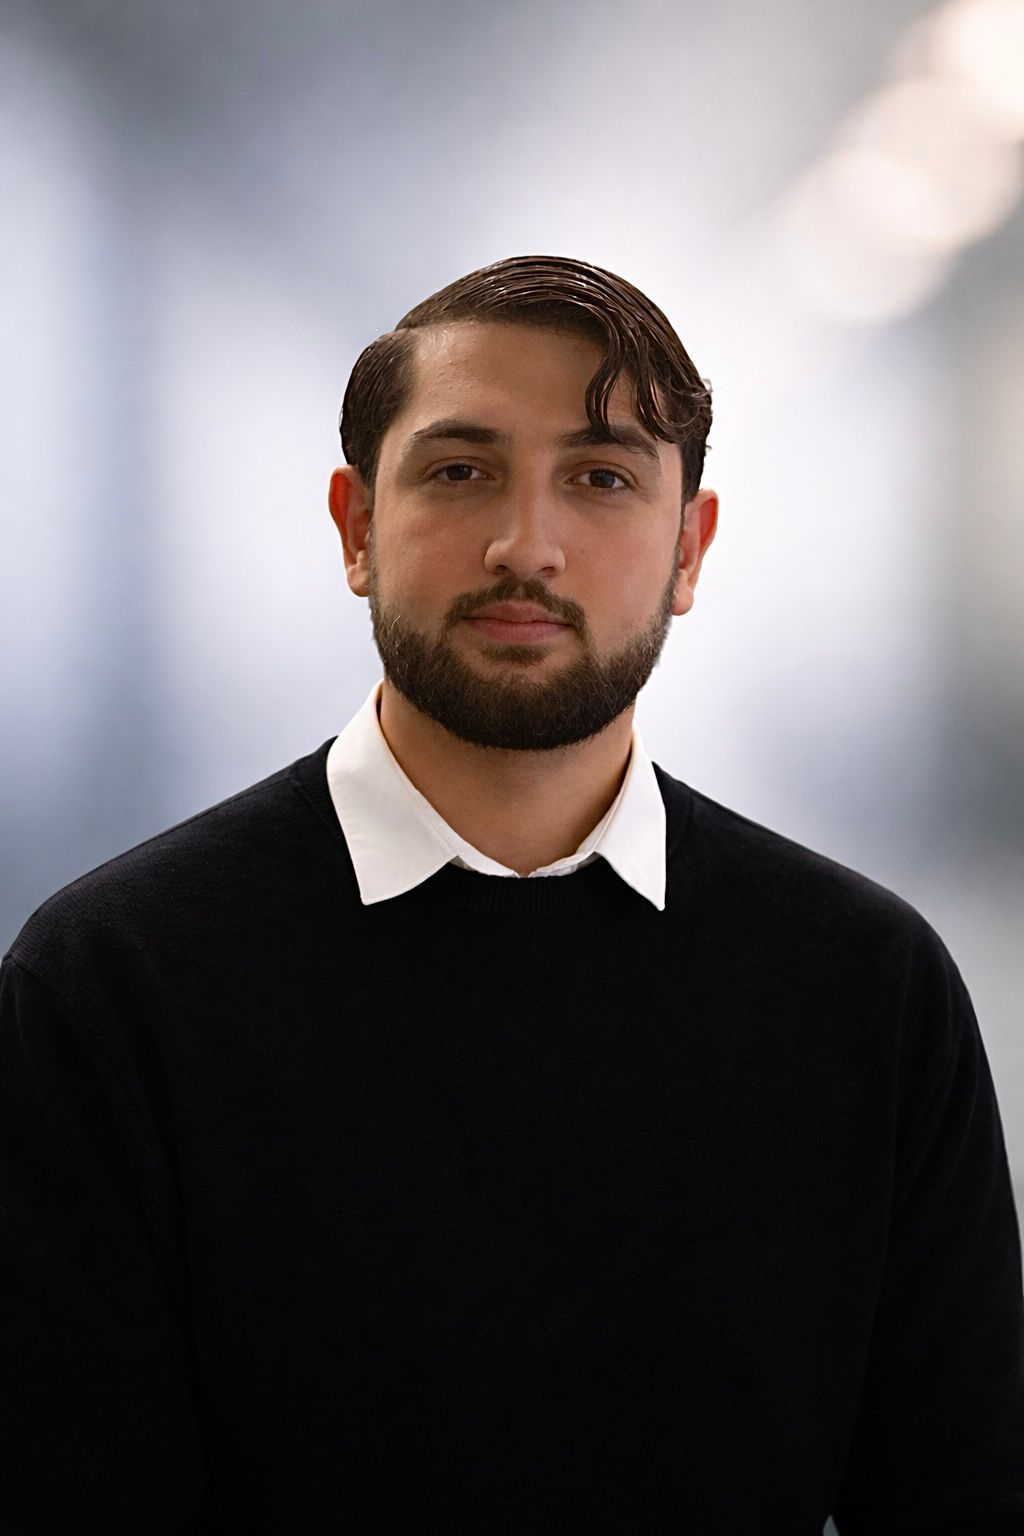
\includegraphics[width=2.4cm]{assets/photo-ozan.jpeg}};
  \end{tikzpicture}
  &
  \begin{tikzpicture}
    \clip (0,0) circle (1.2cm);
    \node at (0,0) {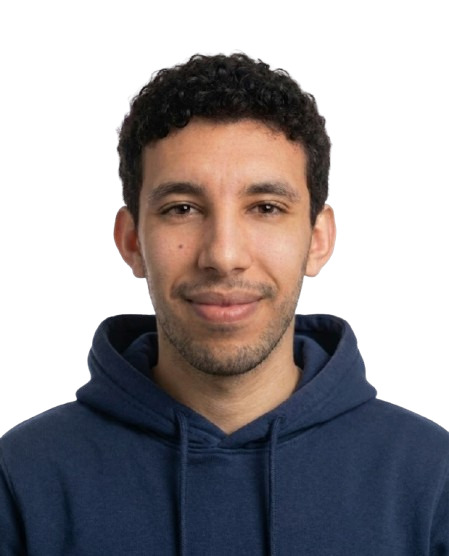
\includegraphics[width=2.4cm]{assets/photo-ales.jpeg}};
  \end{tikzpicture}
  &
  \begin{tikzpicture}
    \clip (0,0) circle (1.2cm);
    \node at (0,0) {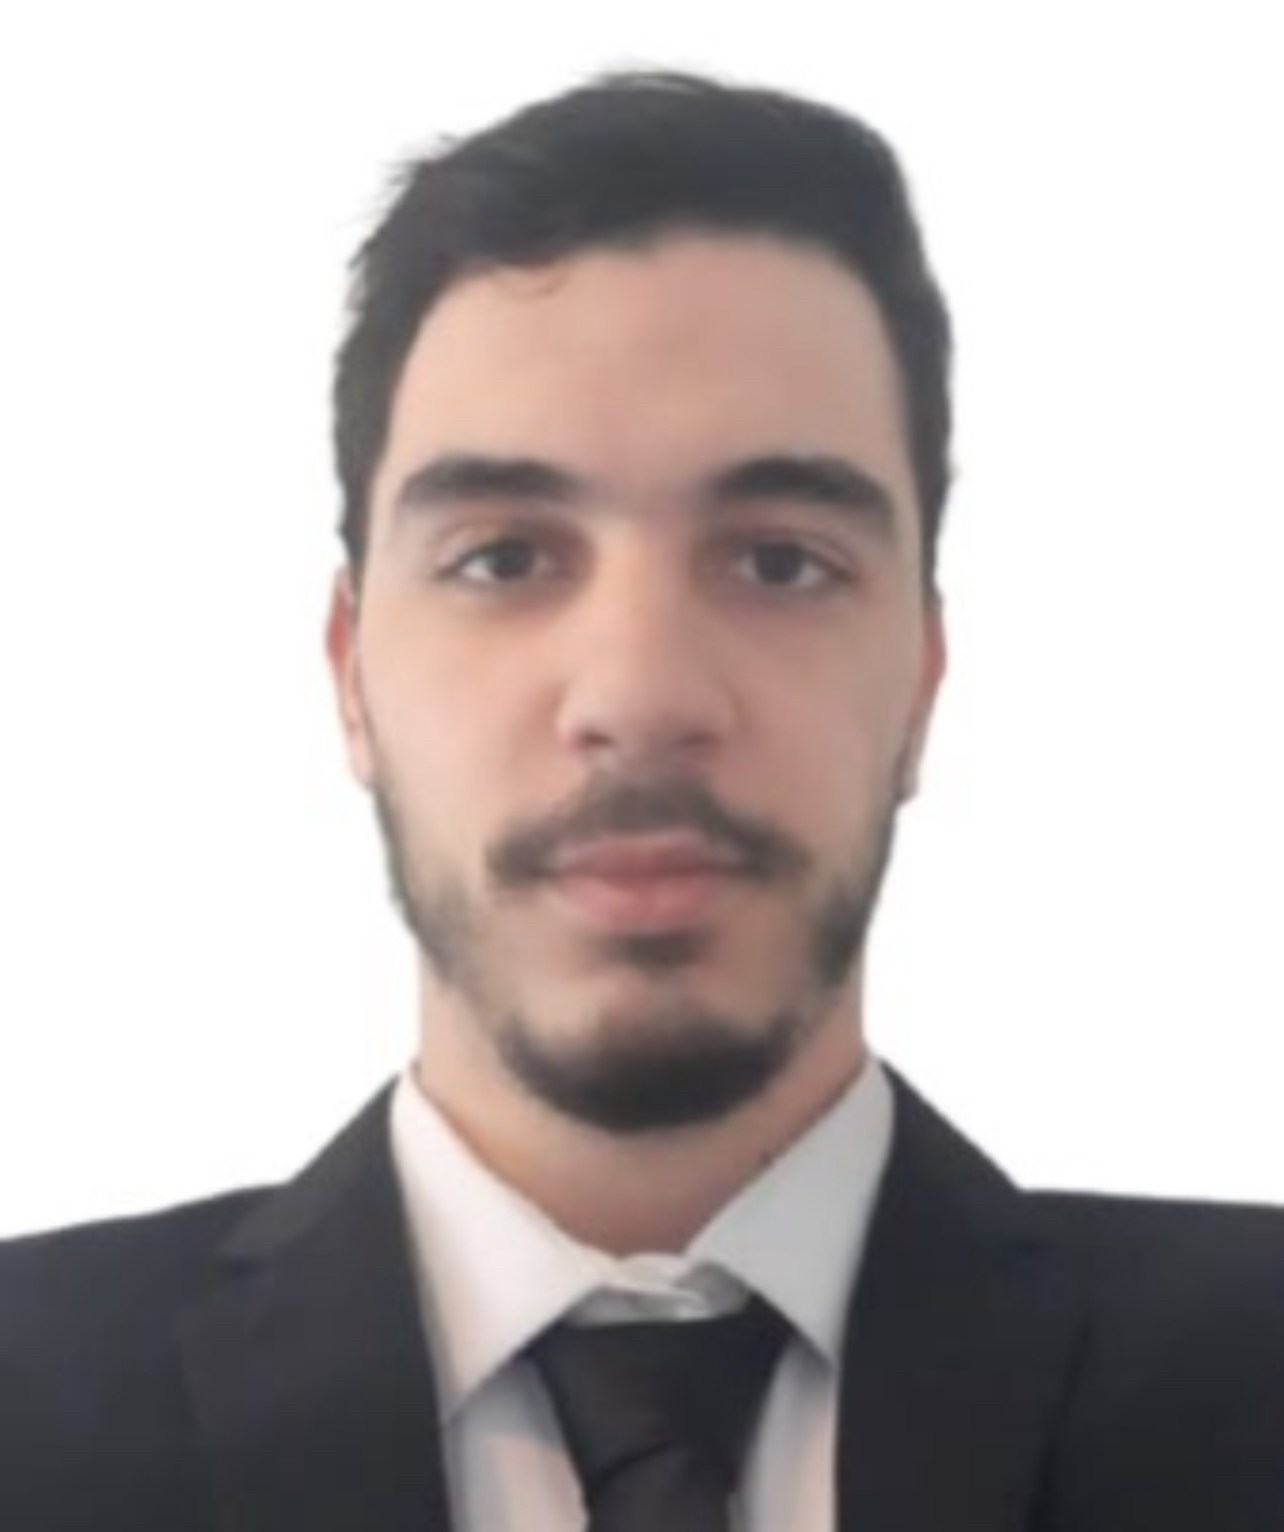
\includegraphics[width=2.4cm]{assets/photo-rayane.jpeg}};
  \end{tikzpicture}
  &
  \begin{tikzpicture}
    \clip (0,0) circle (1.2cm);
    \node at (0,0) {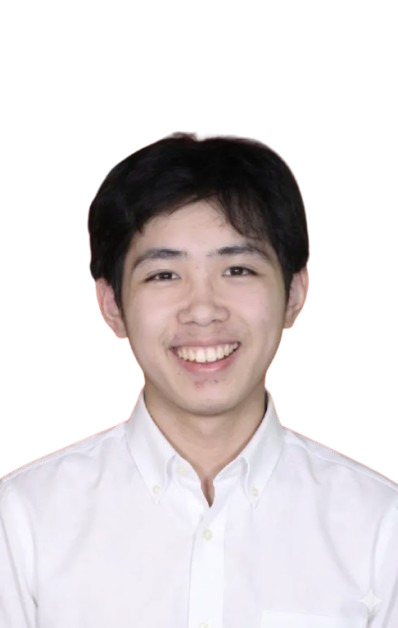
\includegraphics[width=2.4cm]{assets/photo-maxime.jpeg}};
  \end{tikzpicture}
  \\[0.4cm]
  \textbf{Taskin Ozan}
  & \textbf{Ferhani Ales}
  & \textbf{Taouache Rayane}
  & \textbf{Huang Maxime} \\[0.1cm]
  \textcolor[HTML]{1B3A6B}{\small AI / Frontend}
  & \textcolor[HTML]{1B3A6B}{\small AI / Test}
  & \textcolor[HTML]{1B3A6B}{\small Backend / Test}
  & \textcolor[HTML]{1B3A6B}{\small Frontend / Backend} \\
\end{tabular}
\end{center}

\vspace{1.5cm}

\begin{minipage}[t]{0.47\textwidth}
\begin{tcolorbox}[
  equal height group=team,
  colback=white, colframe=gray!50,
  boxrule=1pt, arc=5pt,
  left=8pt, right=8pt, top=8pt, bottom=8pt,
  borderline west={3pt}{0pt}{[HTML]{1E293B}}
]
{\small\textcolor[HTML]{64748B}{IA / Frontend}}\\[0.2cm]
\textbf{Taskin Ozan}\\[0.15cm]
{\small Architecture du système, pipeline CBIR,
fine-tuning BioMedCLIP, interface React.}
\end{tcolorbox}
\end{minipage}
\hfill
\begin{minipage}[t]{0.47\textwidth}
\begin{tcolorbox}[
  equal height group=team,
  colback=white, colframe=gray!50,
  boxrule=1pt, arc=5pt,
  left=8pt, right=8pt, top=8pt, bottom=8pt,
  borderline west={3pt}{0pt}{[HTML]{1E293B}}
]
{\small\textcolor[HTML]{64748B}{IA / Test}}\\[0.2cm]
\textbf{Ferhani Ales}\\[0.15cm]
{\small Scripts d'évaluation, stratégie de tests, traitement embeddings, gouvernance des données.}
\end{tcolorbox}
\end{minipage}

\vspace{1.2cm}

\begin{minipage}[t]{0.47\textwidth}
\begin{tcolorbox}[
  equal height group=team,
  colback=white, colframe=gray!50,
  boxrule=1pt, arc=5pt,
  left=8pt, right=8pt, top=8pt, bottom=8pt,
  borderline west={3pt}{0pt}{[HTML]{1E293B}}
]
{\small\textcolor[HTML]{64748B}{Backend / Test}}\\[0.2cm]
\textbf{Taouache Rayane}\\[0.15cm]
{\small API FastAPI, services backend, déploiement VPS, tests unitaires.}
\end{tcolorbox}
\end{minipage}
\hfill
\begin{minipage}[t]{0.47\textwidth}
\begin{tcolorbox}[
  equal height group=team,
  colback=white, colframe=gray!50,
  boxrule=1pt, arc=5pt,
  left=8pt, right=8pt, top=8pt, bottom=8pt,
  borderline west={3pt}{0pt}{[HTML]{1E293B}}
]
{\small\textcolor[HTML]{64748B}{Frontend / Backend}}\\[0.2cm]
\textbf{Huang Maxime}\\[0.15cm]
{\small Interface React, pipeline et prétraitement des données, services backend, tests frontend.}
\end{tcolorbox}
\end{minipage}

\vspace{1.5cm}

\noindent Le projet a été développé \textbf{collectivement} : chaque membre a contribué
à l'ensemble des composants du système. Naturellement, au fil du projet, des expertises
se sont constituées au sein de l'équipe, reflétées dans la répartition des rôles ci-dessus.

% =========================================================
% SOMMAIRE
% =========================================================
\newpage
\begingroup
\setlength{\columnsep}{1cm}
\renewcommand{\baselinestretch}{1.1}\fontsize{11pt}{13pt}\selectfont
\begin{multicols}{2}
\tableofcontents
\end{multicols}
\endgroup

% =========================================================
% LISTE DES ILLUSTRATIONS
% =========================================================
\newpage
\listoffigures
\listoftables

% =========================================================
% GUIDE DE LECTURE
% =========================================================
\newpage
\section*{Guide de lecture}
\addcontentsline{toc}{section}{Guide de lecture}

\vspace{0.3cm}

Ce rapport documente le cycle complet de réalisation de \textbf{MEDISCAN AI},
de la définition de la problématique jusqu'au déploiement en production.
Plusieurs parcours de lecture sont proposés ci-dessous selon le profil du lecteur.

\vspace{0.3cm}
Le \textbf{Résumé exécutif} constitue le \textbf{point d'entrée commun à tous les lecteurs}
et donne une vision globale du projet en une page.

\vspace{0.6cm}

\textbf{Manager ou décideur : vision stratégique}

\vspace{0.15cm}
Pour saisir la valeur du projet sans entrer dans les détails techniques.
\begin{sq}
  \item \textbf{Section 1} : contexte, enjeux et approche
  \item \textbf{Section 4} : produit déployé et cas d'usage
  \item \textbf{Sections 9 et 11} : bilan et perspectives
\end{sq}

\vspace{0.6cm}

\textbf{Encadrant technique : architecture et réalisation}

\vspace{0.15cm}
Pour évaluer les choix techniques et la qualité de l'implémentation.
\begin{sq}
  \item \textbf{Section 2} : benchmark et positionnement
  \item \textbf{Section 5} : technologies clés et architecture
  \item \textbf{Section 6} : déploiement et infrastructure
  \item \textbf{Section 10} : impact des IA agentiques
  \item \textbf{Annexe A} : documentation API REST
\end{sq}

\vspace{0.6cm}

\textbf{Encadrant pédagogique : rigueur et méthode}

\vspace{0.15cm}
Pour apprécier la démarche projet et la méthodologie d'évaluation.
\begin{sq}
  \item \textbf{Section 3} : gestion de projet et planning
  \item \textbf{Section 7} : évaluation et résultats
  \item \textbf{Section 8} : difficultés rencontrées
\end{sq}

\vspace{0.6cm}

\textbf{Lecteur externe : fonctionnalités et positionnement}

\vspace{0.15cm}
Pour comprendre ce que fait le système et comment il se distingue.
\begin{sq}
  \item \textbf{Sections 1 et 2} : contexte et paysage concurrentiel
  \item \textbf{Section 4} : produit, ergonomie et cas d'usage
\end{sq}

\vspace{0.6cm}

Le \textbf{glossaire} (Annexe D) définit les termes spécialisés du rapport.

% =========================================================
% CHAPITRE 1 — Introduction
% =========================================================
\NewMajorPart
\section*{Résumé exécutif}
\addcontentsline{toc}{section}{Résumé exécutif}

\textbf{MEDISCAN AI} est une plateforme de recherche d'images médicales par le contenu,
développée par l'équipe L3X1 à l'Université Paris Cité.
Elle est \textbf{aujourd'hui en production} sur \url{https://mediscan-ai.site}.

\vspace{0.6cm}
\textbf{Contexte}

\vspace{0.15cm}
Les outils actuels, notamment les systèmes \textbf{PACS}, reposent sur des mots-clés
et ne permettent pas de retrouver un cas similaire à partir d'une image de référence.
Les Vision Transformers récents ouvrent la voie à une recherche par similarité visuelle et sémantique.

\vspace{0.6cm}
\textbf{Solution}

\vspace{0.15cm}
\begin{sq}
  \item Moteur de recherche combinant deux approches complémentaires : similarité visuelle et analyse du contenu médical.
  \item Trois modes d'usage : \textbf{par image} (analyse visuelle), \textbf{par image} (sens clinique) et \textbf{par description textuelle}.
  \item Une synthèse automatique résume les résultats et met en évidence les tendances communes.
\end{sq}

\vspace{0.6cm}
\textbf{Architecture}

\vspace{0.15cm}
\begin{sq}
  \item \textbf{Confidentialité :} aucune donnée ne quitte l'infrastructure de l'équipe.
  \item \textbf{Accessibilité :} interface web sans installation, disponible 24h/24.
  \item \textbf{Couverture :} index de \textbf{60\,000 images médicales} référencées.
\end{sq}

\vspace{0.6cm}
\textbf{Résultats}

\vspace{0.15cm}
Le système retrouve des cas pertinents et exploitables dans plus de \textbf{88\,\%} des situations,
validé sur un jeu de \textbf{9\,000 requêtes} couvrant l'ensemble des modes de recherche.

\vspace{0.6cm}
\textbf{Cadre d'usage}

\vspace{0.15cm}
\textbf{MEDISCAN AI} est un prototype académique non clinique : il ne pose aucun diagnostic
et ne remplace pas un professionnel de santé.

\vspace{0.6cm}
\textbf{Perspectives}

\vspace{0.15cm}
\begin{sq}
  \item Intégration native du format \textbf{DICOM} et fine-tuning sur données internes.
  \item Mise en place d'un pipeline \textbf{CI/CD} pour automatiser les déploiements.
\end{sq}
% =========================================================
% CHAPITRE 1 — Contexte et enjeux
% =========================================================
\NewMajorPart
\section{Contexte et enjeux}

\vspace{0.2cm}
Cette section présente le cadre dans lequel s'inscrit \textbf{MEDISCAN AI},
la problématique qu'il adresse et l'approche retenue par l'équipe.

\vspace{0.5cm}

\subsection{Contexte métier et motivation}

\vspace{0.2cm}
La recherche d'images médicales par le contenu visuel est l'un des apports concrets des nouvelles technologies
appliquées à la santé. Elle ouvre des perspectives utiles à différents profils d'utilisateurs.

\vspace{0.2cm}
\begin{sq}
  \item Un médecin peut retrouver rapidement des cas antérieurs similaires pour appuyer son analyse.
  \item Un étudiant peut explorer un corpus d'images sous différents angles pour enrichir sa formation.
  \item Un chercheur peut naviguer efficacement dans de grands ensembles d'images médicales.
\end{sq}

\vspace{0.5cm}

\subsection{Problématique}

\vspace{0.2cm}
\begin{tcolorbox}[colback=gray!8, colframe=gray!40, boxrule=0.4pt, arc=2pt]
\textbf{\textit{Comment rendre praticable la recherche d'images médicales pertinentes
dans de larges corpus, sans dépendre exclusivement d'annotations manuelles
et dans le respect de la confidentialité des données ?}}
\end{tcolorbox}

\vspace{0.5cm}

\subsection{Notre approche}

\vspace{0.2cm}
Plutôt que de s'appuyer uniquement sur des mots-clés, nous avons fait le choix
d'une recherche multimodale : l'utilisateur peut interroger le système par l'image
ou par une description textuelle, selon son besoin.

\vspace{0.2cm}
\begin{sq}
  \item Deux moteurs complémentaires couvrent la similarité visuelle et le sens clinique.
  \item L'interface permet de comparer, filtrer et affiner les résultats sans relancer de recherche.
  \item Une synthèse automatique aide à interpréter les résultats retournés.
\end{sq}


% =========================================================
% CHAPITRE 2 — Benchmark
% =========================================================
\NewMajorPart
\section{Benchmark et positionnement}

Cette section situe \textbf{MEDISCAN AI} face aux solutions existantes en imagerie médicale.

\subsection{Recherche d'images par le contenu (CBIR)}

Le \textbf{CBIR} (\textit{Content-Based Image Retrieval}) désigne la recherche d'images
par leur contenu plutôt que par mots-clés. Les approches modernes fondées sur
l'apprentissage profond permettent de capturer à la fois la similarité visuelle
et le sens clinique d'une image.

\subsection{Solutions existantes et analyse comparative}

Comparaison de \textbf{MEDISCAN AI} avec les systèmes de \textbf{CBIR médical}
et les principales plateformes d'imagerie médicale connues.

\begin{table}[H]
\centering
\renewcommand{\arraystretch}{1.15}
\footnotesize
\begin{tabularx}{\textwidth}{@{}>{\raggedright\arraybackslash}p{3.5cm}*{7}{>{\centering\arraybackslash}X}@{}}
\toprule
\textbf{Système} &
\rotatebox{55}{\scriptsize\textbf{Recherche visuelle}} &
\rotatebox{55}{\scriptsize\textbf{Recherche sémantique}} &
\rotatebox{55}{\scriptsize\textbf{Recherche textuelle}} &
\rotatebox{55}{\scriptsize\textbf{Comparaison}} &
\rotatebox{55}{\scriptsize\textbf{Synthèse IA}} &
\rotatebox{55}{\scriptsize\textbf{Interface produit}} &
\rotatebox{55}{\scriptsize\textbf{Confidentialité}} \\
\midrule
\rowcolor{gray!15} \textbf{MEDISCAN AI} & \cmark & \cmark & \cmark & \cmark & \cmark & \cmark & \cmark \\
Yottixel             & \cmark & \xmark & \xmark & \xmark & \xmark & \cmark & \cmark \\
\midrule
OpenI (NLM)          & \xmark & \xmark & \cmark & \xmark & \xmark & \cmark & \xmark \\
MedGemma             & \xmark & \xmark & \cmark & \xmark & \cmark & \cmark & \xmark \\
MONAI (NVIDIA)       & \xmark & \xmark & \xmark & \xmark & \xmark & \cmark & \cmark \\
Aidoc                & \xmark & \xmark & \xmark & \xmark & \cmark & \cmark & \xmark \\
\bottomrule
\end{tabularx}
\caption{Comparaison de MEDISCAN AI avec les principales plateformes d'imagerie médicale}
\label{tab:benchmark}
\end{table}

\subsection{Un terrain d'opportunité pour la recherche}

Les systèmes \textbf{PACS} déployés dans les hôpitaux ne disposent pas de recherche
par le contenu visuel : les requêtes restent limitées aux métadonnées textuelles.
L'intégration d'un moteur multimodal comme \textbf{MEDISCAN AI} constitue ainsi un
terrain d'expérimentation prometteur pour la recherche en imagerie médicale.

% =========================================================
% CHAPITRE 3 — Gestion de projet
% =========================================================
\NewMajorPart
\section{Gestion de projet}

Cette section présente la méthodologie de travail adoptée par l'équipe L3X1
et le planning du projet.

\vspace{0.4cm}

\subsection{Méthodologie}

\vspace{0.2cm}
L'équipe a adopté un cycle \textbf{incrémental} inspiré des méthodes agiles.

\vspace{0.2cm}
\begin{sq}
  \item \textbf{Incréments} : quatre livrables successifs : cœur CBIR, API backend,
        interface frontend, fine-tuning et évaluation.
  \item \textbf{Versionnement} : branches de fonctionnalité sur \textbf{SVN},
        vérification avant chaque fusion sur la branche principale.
  \item \textbf{Coordination} : points de synchronisation bi-quotidiens sur \textbf{Discord}.
\end{sq}

\vspace{0.7cm}

\subsection{Planning et jalons}

\vspace{0.2cm}
Le projet s'est déroulé sur un semestre, structuré en quatre phases successives.

\vspace{0.2cm}
\begin{sq}
  \item \textbf{Phase 1} : analyse des besoins, choix techniques et mise en place
        de l'environnement de développement.
  \item \textbf{Phase 2} : implémentation du cœur CBIR : embedders, index FAISS,
        pipeline de recherche et API backend.
  \item \textbf{Phase 3} : développement de l'interface React, intégration
        frontend-backend et fine-tuning de BioMedCLIP sur ROCOv2.
  \item \textbf{Phase 4} : évaluation, tests, déploiement VPS et rédaction du rapport.
\end{sq}

\vspace{0.5cm}

\begin{figure}[H]
  \centering
  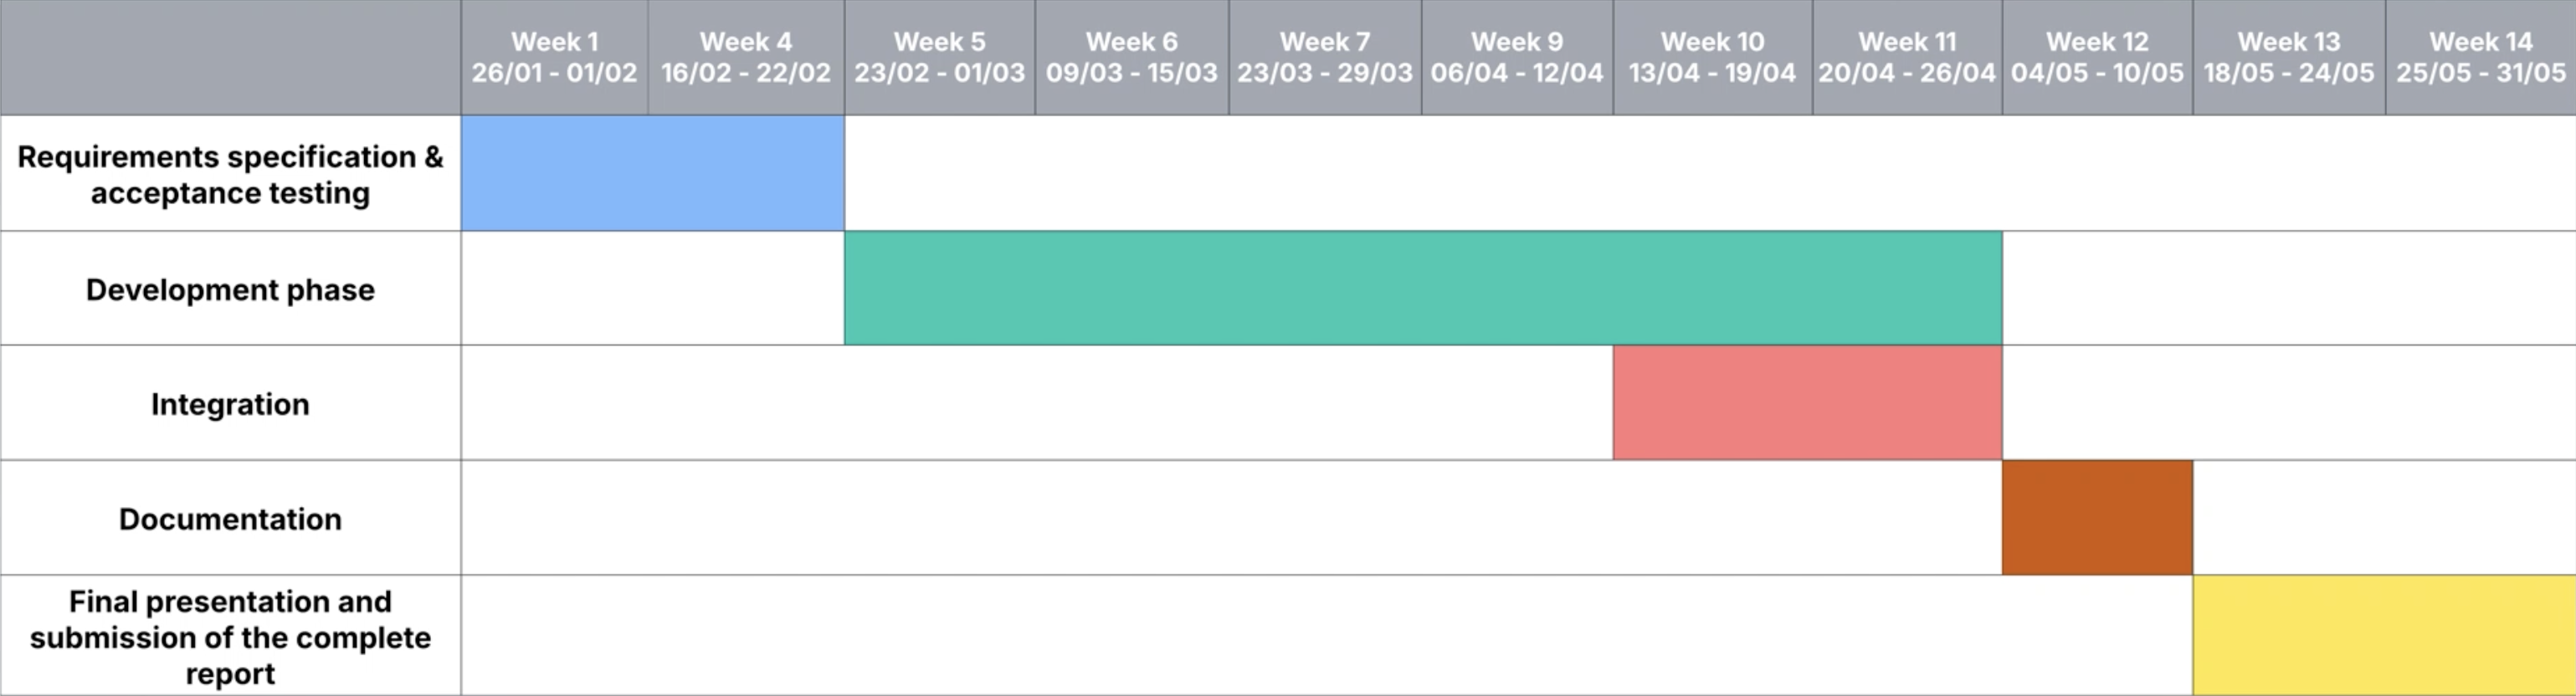
\includegraphics[width=\textwidth]{assets/gantt.png}
  \caption{Planning du projet MEDISCAN AI}
  \label{fig:gantt}
\end{figure}


% =========================================================
% CHAPITRE 4 — Cahier des charges
% =========================================================
\NewMajorPart
\section{Produit}

Cette section présente \textbf{MEDISCAN AI} en tant que produit déployé :
sa réponse concrète à la problématique posée et les cas d'usage rendus possibles
par la version aujourd'hui en ligne.

\vspace{0.5cm}

\subsection{Réponse à la problématique}

\vspace{0.2cm}
\begin{tcolorbox}[colback=gray!8, colframe=gray!40, boxrule=0.4pt, arc=2pt]
\textbf{\textit{Comment rendre praticable la recherche d'images médicales pertinentes
dans de larges corpus, sans dépendre exclusivement d'annotations manuelles
et dans le respect de la confidentialité des données ?}}
\end{tcolorbox}

\vspace{0.3cm}
\textbf{MEDISCAN AI} répond à cette problématique sur trois axes complémentaires.

\vspace{0.3cm}

\begin{sq}
  \item \textbf{Rapidité} : optimisations sur l'index vectoriel et le traitement des données pour des réponses en quelques centaines de millisecondes.
  \item \textbf{Pertinence} : un corpus de référence de \textbf{60\,000 images} issues du dataset public \textbf{ROCOv2}, couvrant un large spectre de modalités et d'organes.
  \item \textbf{Interopérabilité / Confidentialité} : architecture pluggable, capable d'indexer n'importe quel corpus interne, déployable localement ou exposée par API, sans transfert vers un service externe.
\end{sq}

\vspace{0.7cm}

\subsection{Cas d'utilisation}

\vspace{0.2cm}
La plateforme est aujourd'hui en ligne sur \url{https://mediscan-ai.site}.
Elle permet, depuis n'importe quel navigateur et sans installation,
plusieurs usages concrets autour de la recherche d'images médicales.

\vspace{0.3cm}

\begin{sq}
  \item \textbf{Recherche par image} : retrouver les cas visuellement ou cliniquement proches d'une image requête.
  \item \textbf{Recherche textuelle} : interroger le corpus à partir d'une description clinique.
  \item \textbf{Comparaison d'images} : confronter côte à côte l'image requête et les résultats retournés.
  \item \textbf{Synthèse exploratoire} : obtenir une interprétation automatique des résultats à des fins d'analyse.
  \item \textbf{Export des résultats} : récupérer les résultats au format JSON, CSV ou PDF.
\end{sq}

\vfill
\raggedright
\newpage
\subsection{Interface et ergonomie}

\begin{figure}[H]
  \centering
  \roundedimg[width=\textwidth]{assets/home.png}
  \caption{Page d'accueil de MEDISCAN AI}
  \label{fig:home}
\end{figure}

\vspace{0.6cm}

\noindent
\begin{minipage}[c]{0.28\textwidth}
  \roundedimg[width=\textwidth]{assets/theme-dark.png}
\end{minipage}
\hfill
\begin{minipage}[c]{0.67\textwidth}
  \vspace{-0.6cm}
  \captionsetup{justification=raggedright, singlelinecheck=false}
  \captionof{figure}{Sélecteur de thème et de langue}
  \vspace{0.2cm}
  {\small L'interface propose un \textbf{thème clair et sombre} adaptable
  à l'environnement de travail, ainsi qu'une bascule de langue
  \textbf{FR / EN} accessible depuis la barre de navigation.}
\end{minipage}

\vspace{0.6cm}

\noindent
\begin{minipage}[c]{0.28\textwidth}
  \parbox[c]{\textwidth}{%
  \raggedright
  {\small Le \textbf{hub central} est le point d'entrée vers les deux pages
  dédiées aux modes de recherche : Visual Search pour la recherche
  par image, et Text Guided Search pour la recherche textuelle.}\par}
\end{minipage}
\hfill
\begin{minipage}[c]{0.68\textwidth}
  \centering
  \roundedimg[width=\textwidth]{assets/hub.png}
  \captionsetup{justification=centering, singlelinecheck=false}
  \captionof{figure}{Hub de sélection du mode de recherche}
\end{minipage}

\newpage
\subsection{Modes de recherche}

\vspace*{0.5cm}
\noindent L'application propose trois modes complémentaires accessibles depuis le hub central.

\vspace{0.8cm}
\noindent
\begin{minipage}[c]{0.65\textwidth}
  \centering
  \roundedimg[width=\textwidth]{assets/visual-analysis.png}
  \captionsetup{justification=centering, singlelinecheck=false}
  \captionof{figure}{Mode Visual Analysis}
\end{minipage}
\hfill
\begin{minipage}[c]{0.31\textwidth}
  \vspace{-0.8cm}
  \raggedright
  {\small L'utilisateur dépose une image médicale.
  Le système retourne les images visuellement proches
  via \textbf{DINOv2} (768D).
  Adapté à la recherche par morphologie et structure anatomique.}
\end{minipage}

\vspace{1.4cm}

\noindent
\begin{minipage}[c]{0.31\textwidth}
  \raggedright
  {\small Recherche par proximité médicale via \textbf{BioMedCLIP} fine-tuné (512D).
  Privilégie le sens clinique sur la ressemblance visuelle.}
\end{minipage}
\hfill
\begin{minipage}[c]{0.65\textwidth}
  \centering
  \roundedimg[width=\textwidth]{assets/interpretive-analysis.png}
  \captionsetup{justification=centering, singlelinecheck=false}
  \captionof{figure}{Mode Interpretive Analysis}
\end{minipage}

\vspace{1.4cm}

\noindent
\begin{minipage}[c]{0.65\textwidth}
  \centering
  \roundedimg[width=\textwidth]{assets/text-query.png}
  \captionsetup{justification=centering, singlelinecheck=false}
  \captionof{figure}{Mode Text Query}
\end{minipage}
\hfill
\begin{minipage}[c]{0.31\textwidth}
  \raggedright
  {\small L'utilisateur saisit une description clinique.
  Le système retourne les images alignées
  via \textbf{BioMedCLIP} (500 caractères max).}
\end{minipage}

\subsection{Résultats et exploration}

\vspace{0.2cm}
\noindent Une fois la recherche lancée, l'interface propose des outils d'exploration
et de relance pour affiner les résultats.

\vfill
\begin{center}
  \roundedimg[width=0.85\textwidth]{assets/result-filter.png}
\end{center}
\captionsetup{justification=centering, singlelinecheck=false}
\captionof{figure}{Grille de résultats avec filtres et scores de similarité}
\vspace{0.15cm}
\noindent{\small Les filtres affinent les résultats sans relancer la recherche :
\textbf{score}, \textbf{caption}, \textbf{CUI} et \textbf{tri}.}
\vspace{0.9cm}
\vfill
\noindent
\begin{minipage}[c]{0.62\textwidth}
  \centering
  \roundedimg[width=\textwidth]{assets/relance.png}
  \captionsetup{justification=centering, singlelinecheck=false}
  \captionof{figure}{Relance de recherche depuis une sélection d'images}
\end{minipage}
\hfill
\begin{minipage}[c]{0.34\textwidth}
  \vspace{-0.8cm}
  \raggedright
  {\small Une \textbf{sélection d'images} devient une \textbf{nouvelle requête}
  via \textbf{centroïde d'embeddings}.
  \begin{num}
    \item Sélectionner une ou plusieurs images.
    \item Relancer depuis la sélection.
  \end{num}}
\end{minipage}
\vfill

\vspace*{1.2cm}
\begin{center}
  \roundedimg[width=0.85\textwidth]{assets/comparaison.png}
\end{center}
\captionsetup{justification=centering, singlelinecheck=false}
\captionof{figure}{Comparaison entre l'image requête et les résultats retournés}
\vspace{0.2cm}
\noindent{\small L'interface affiche \textbf{côte à côte} l'\textbf{image requête} et les
\textbf{résultats retournés}, permettant une \textbf{comparaison visuelle directe}.}

\vspace{1.2cm}
\vfill
\noindent
\begin{minipage}[c]{0.34\textwidth}
  \raggedright
  {\small Le \textbf{module de synthèse} analyse les résultats et génère
  une \textbf{interprétation exploratoire} assistée par IA.}
  \vspace{0.3cm}
  {\small
  \begin{num}
    \item Synthèse générée via \textbf{Groq} à partir des captions des résultats.
    \item Identifie les \textbf{patterns récurrents} sans poser de diagnostic.
  \end{num}}
\end{minipage}
\hfill
\begin{minipage}[c]{0.62\textwidth}
  \centering
  \roundedimg[width=\textwidth]{assets/ai_summary.png}
  \captionsetup{justification=centering, singlelinecheck=false}
  \captionof{figure}{Synthèse exploratoire générée par IA}
\end{minipage}
\vfill

% =========================================================
% CHAPITRE 5 — Technologies clés
% =========================================================
\NewMajorPart
\section{Technologies clés}

\vspace{0.2cm}
\textbf{MEDISCAN AI} s'appuie sur deux modèles d'IA aux architectures complémentaires,
combinés à un moteur de recherche vectorielle haute performance.

\subsection{Architecture des pipelines d'embedding}

\vspace{0.3cm}
\begin{figure}[H]
  \centering
  \roundedimg[width=\textwidth]{assets/archi.png}
  \caption{Architecture des deux pipelines d'embedding — BioMedCLIP (sémantique) et DINOv2 (visuel)}
  \label{fig:archi}
\end{figure}

\vspace{0.5cm}

\noindent
\begin{minipage}[t]{0.47\textwidth}
  \textbf{BioMedCLIP} (512D)\\[0.3cm]
  Architecture duale : un encodeur image (ViT) et un encodeur texte (Transformer)
  entraînés conjointement sur 15 millions de paires image-texte biomédicales.
  \vspace{0.2cm}
  \begin{sq}[leftmargin=1.2em]
    \item Aligne images et textes dans un espace vectoriel commun.
    \item Utilisé pour les modes \textbf{Interpretive Analysis} et \textbf{Text Guided Search}.
  \end{sq}
\end{minipage}
\hfill
\begin{minipage}[t]{0.47\textwidth}
  \textbf{DINOv2} (768D)\\[0.3cm]
  Vision Transformer (ViT-L/14) pré-entraîné de manière auto-supervisée
  sur 142 millions d'images sans annotation.
  \vspace{0.2cm}
  \begin{sq}[leftmargin=1.2em]
    \item Capture structures visuelles, textures et morphologie.
    \item Utilisé pour le mode \textbf{Visual Search}.
  \end{sq}
\end{minipage}

\vspace{0.6cm}

\noindent\textbf{Fine-tuning de BioMedCLIP.}
Le modèle a été ré-entraîné sur le dataset \textbf{ROCOv2} pendant plusieurs epochs
afin d'y adapter ses représentations.

\vspace{0.5cm}

\subsection{Technologies de développement}

\vspace{0.2cm}
Stack moderne organisée en trois blocs : frontend, backend et couche IA.

\vspace{0.4cm}

\noindent
\begin{minipage}[t]{0.31\textwidth}
  \centering
  \textbf{Frontend}\\[0.3cm]
  \begin{minipage}[t][1.2cm][c]{\textwidth}
    \centering
    \makebox[1.5cm][c]{
\includegraphics[width=1.3cm,height=1cm,keepaspectratio]{assets/react.png}}%
    \makebox[1.5cm][c]{
\includegraphics[width=1.3cm,height=1cm,keepaspectratio]{assets/tailwind.png}}%
    \makebox[1.5cm][c]{
\includegraphics[width=1.3cm,height=1cm,keepaspectratio]{assets/vite.jpeg}}
  \end{minipage}\\[0.3cm]
  {\small Construction de l'\textbf{interface utilisateur} et de l'expérience visuelle.}
\end{minipage}
\hfill
\begin{minipage}[t]{0.31\textwidth}
  \centering
  \textbf{Backend}\\[0.3cm]
  \begin{minipage}[t][1.2cm][c]{\textwidth}
    \centering
    \makebox[1.5cm][c]{
\includegraphics[width=1.3cm,height=1cm,keepaspectratio]{assets/python.png}}%
    \makebox[1.5cm][c]{
\includegraphics[width=1.3cm,height=1cm,keepaspectratio]{assets/fastapi.png}}%
    \makebox[1.5cm][c]{
\includegraphics[width=1.3cm,height=1cm,keepaspectratio]{assets/mongodb.png}}
  \end{minipage}\\[0.3cm]
  {\small \textbf{Pont entre l'interface et l'IA}, gestion des requêtes et données.}
\end{minipage}
\hfill
\begin{minipage}[t]{0.31\textwidth}
  \centering
  \textbf{Core AI}\\[0.3cm]
  \begin{minipage}[t][1.2cm][c]{\textwidth}
    \centering
    \makebox[1.5cm][c]{
\includegraphics[width=1.3cm,height=1cm,keepaspectratio]{assets/pytorch.png}}%
    \makebox[1.5cm][c]{
\includegraphics[width=1.3cm,height=1cm,keepaspectratio]{assets/meta.png}}%
    \makebox[1.5cm][c]{
\includegraphics[width=1.3cm,height=1cm,keepaspectratio]{assets/microsoft.png}}
  \end{minipage}\\[0.3cm]
  {\small \textbf{Analyse et compréhension} des images médicales pour la recherche par contenu.}
\end{minipage}

\vspace{0.5cm}

\subsection{FAISS et optimisation de la recherche}

\vspace{0.2cm}
La recherche vectorielle repose sur \textbf{FAISS} (\textit{Facebook AI Similarity Search}).

\vspace{0.15cm}
\begin{sq}
  \item Index \textbf{FlatIP} sur \textbf{60\,000 vecteurs} : recherche exacte en quelques ms.
  \item Chargement \textit{lazy} des modèles et de l'index pour limiter la mémoire.
  \item Architecture \textit{stateless} : passage à l'échelle vers plusieurs millions d'images.
\end{sq}

\vspace{0.5cm}

\subsection{Stockage cloud et infrastructure d'entraînement}

\vspace{0.2cm}
Deux ressources externes complémentaires : \textbf{Hugging Face} pour les données,
\textbf{Kaggle} pour le calcul.

\vspace{0.4cm}

\noindent
\begin{minipage}[t]{0.47\textwidth}
  \centering
  
\includegraphics[height=1.3cm]{assets/huggingface.png}\\[0.3cm]
  \raggedright
  \textbf{Hugging Face} : \textit{Stockage cloud}
  \vspace{0.15cm}

  {\small Plateforme essentielle qui héberge l'ensemble des \textbf{60\,000 images}
  du dataset \textbf{ROCOv2}. Elle permet un accès à la demande, sans dupliquer
  le corpus en local, tout en garantissant l'unicité de la version utilisée
  par l'équipe et un déploiement allégé.}
\end{minipage}
\hfill
\begin{minipage}[t]{0.47\textwidth}
  \centering
  
\includegraphics[height=1.3cm]{assets/kaggle.png}\\[0.3cm]
  \raggedright
  \textbf{Kaggle} : \textit{GPU d'entraînement}
  \vspace{0.15cm}

  {\small Ressource clé pour le \textbf{fine-tuning de BioMedCLIP}.
  Les GPU mis à disposition gratuitement par Kaggle ont permis d'entraîner
  les modèles sans investir dans une infrastructure matérielle dédiée,
  ouvrant la voie à des itérations rapides.}
\end{minipage}

% =========================================================
% CHAPITRE 6 — Déploiement et exploitation
% =========================================================
\NewMajorPart
\section{Déploiement et exploitation}

\vspace{0.2cm}
Cette section présente l'infrastructure mise en place pour rendre \textbf{MEDISCAN AI}
accessible en production, ainsi que les choix garantissant sa stabilité et son évolutivité.

\subsection{Architecture et pipeline de déploiement}

\vspace{0.2cm}
L'application est déployée sur un \textbf{VPS Hostinger},
accessible via \texttt{mediscan-ai.site}.

\begin{sq}
  \item \textbf{Nginx} - reverse proxy, routage des requêtes frontend et backend.
  \item \textbf{Gunicorn + Uvicorn} - serveur ASGI pour l'API FastAPI.
  \item \textbf{systemd} - gestion des services et redémarrage automatique.
\end{sq}

\vspace{0.2cm}
Le déploiement suit un pipeline en quatre étapes.

\begin{num}
  \item Configuration du serveur Linux : mises à jour, firewall, ports 80/443.
  \item Installation des dépendances backend et build du frontend (Vite).
  \item Configuration Nginx avec virtual host et certificat SSL.
  \item Activation des services systemd pour le backend et le frontend.
\end{num}

\subsection{Production, accessibilité et évolutivité}

\vspace{0.2cm}
\textbf{MEDISCAN AI} est déployé en production et utilisable depuis n'importe quel navigateur,
sans installation côté utilisateur.

\begin{sq}
  \item \textbf{Accessibilité} - le service est disponible 24h/24 via
        \texttt{mediscan-ai.site}, avec connexion chiffrée HTTPS.
  \item \textbf{Confidentialité} - aucune image n'est transmise à un service externe ;
        tout le traitement s'effectue sur le serveur de l'équipe.
  \item \textbf{Stabilité} - le redémarrage automatique (systemd) garantit
        la continuité du service en cas d'arrêt inattendu.
\end{sq}

\vspace{0.2cm}
L'architecture choisie permet une montée en charge progressive.

\begin{sq}
  \item L'index FAISS est conçu pour passer de 60\,000 à plusieurs millions d'images
        sans modifier l'interface ni l'API.
  \item Le backend FastAPI est sans état (\textit{stateless}) : plusieurs instances
        peuvent être déployées en parallèle derrière Nginx pour absorber la charge.
  \item L'ajout d'un nouveau mode de recherche ou d'un nouveau modèle d'embedding
        ne nécessite pas de refonte de l'architecture.
\end{sq}

% =========================================================
% CHAPITRE 7 — Évaluation et résultats
% =========================================================
\NewMajorPart
\section{Évaluation et résultats}

\vspace{0.2cm}
L'équipe a pu s'appuyer sur des \textbf{annotations manuelles} produites par des
\textbf{doctorants en imagerie médicale}, fournissant une vérité terrain experte
(\textbf{modalité}, \textbf{organe}, \textbf{région anatomique}). Plus de \textbf{9\,000 requêtes}
ont ainsi été évaluées sur les deux moteurs.

\vspace{0.5cm}

\subsection{Résultats du moteur visuel (DINOv2)}

\vspace{0.3cm}

\noindent
\begin{minipage}[t]{0.48\textwidth}
  \centering
  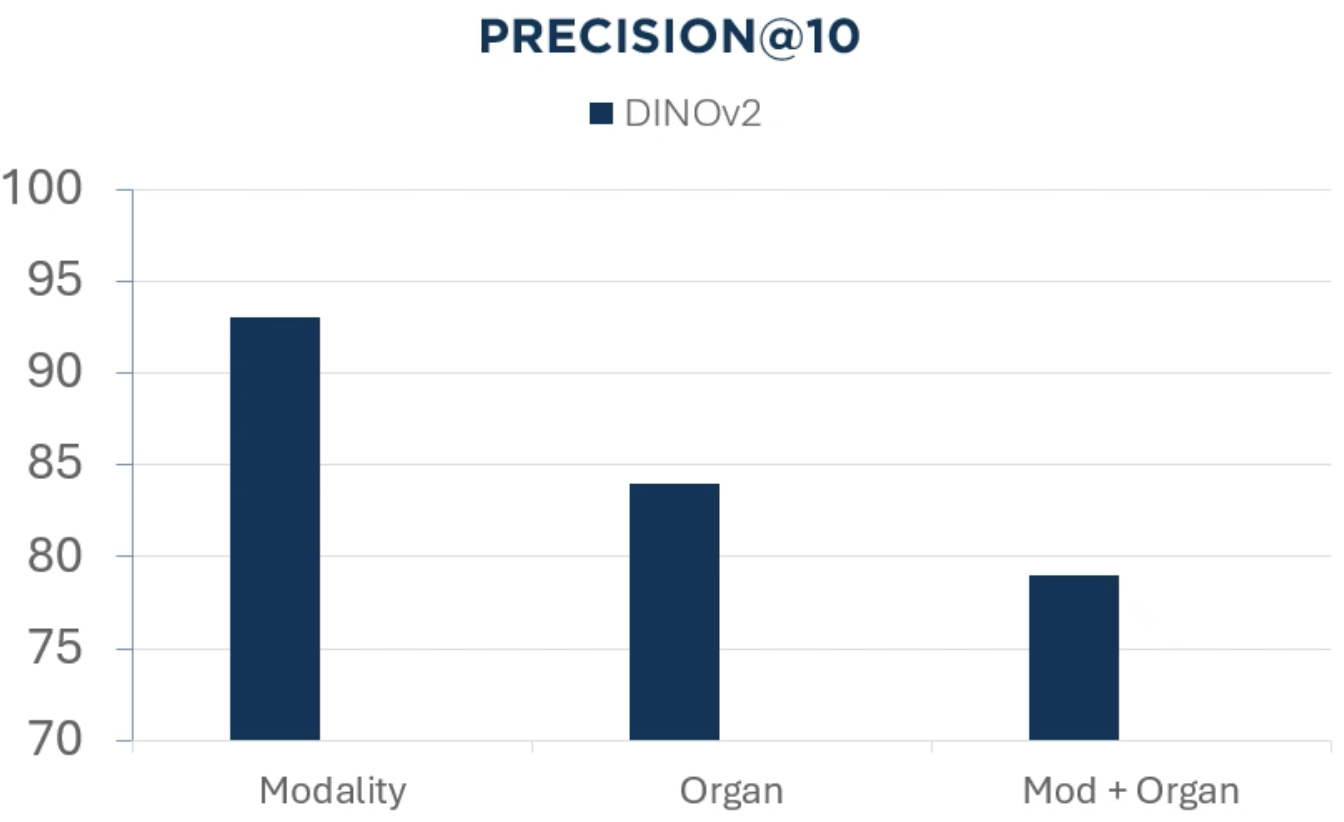
\includegraphics[width=\textwidth]{assets/dinov2Prec.png}
  \captionsetup{justification=centering, singlelinecheck=false}
  \captionof{figure}{DINOv2 : Precision@k}
\end{minipage}
\hfill
\begin{minipage}[t]{0.48\textwidth}
  \centering
  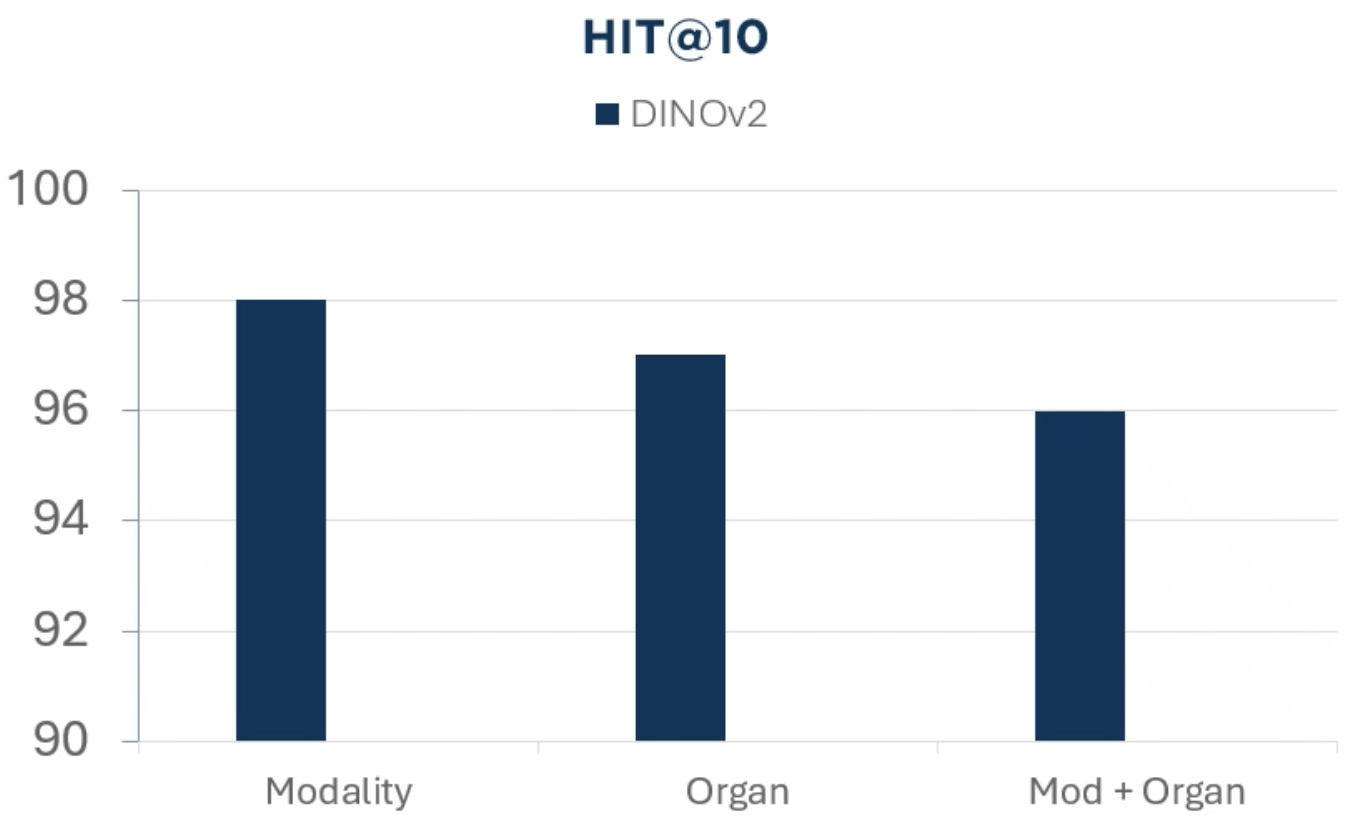
\includegraphics[width=\textwidth]{assets/dinov2HIT.png}
  \captionsetup{justification=centering, singlelinecheck=false}
  \captionof{figure}{DINOv2 : Hit@k}
\end{minipage}

\vspace{0.3cm}
\noindent{\small\textbf{Interprétation.}
DINOv2 obtient une \textbf{Precision} élevée sur la modalité et l'anatomie, confirmant
qu'il capture efficacement les structures visuelles. Le \textbf{Hit@k} valide son usage
pour la recherche par similarité visuelle.}

\vspace{0.5cm}

\subsection{Résultats du moteur sémantique (BioMedCLIP)}

\vspace{0.3cm}

\noindent
\begin{minipage}[t]{0.48\textwidth}
  \centering
  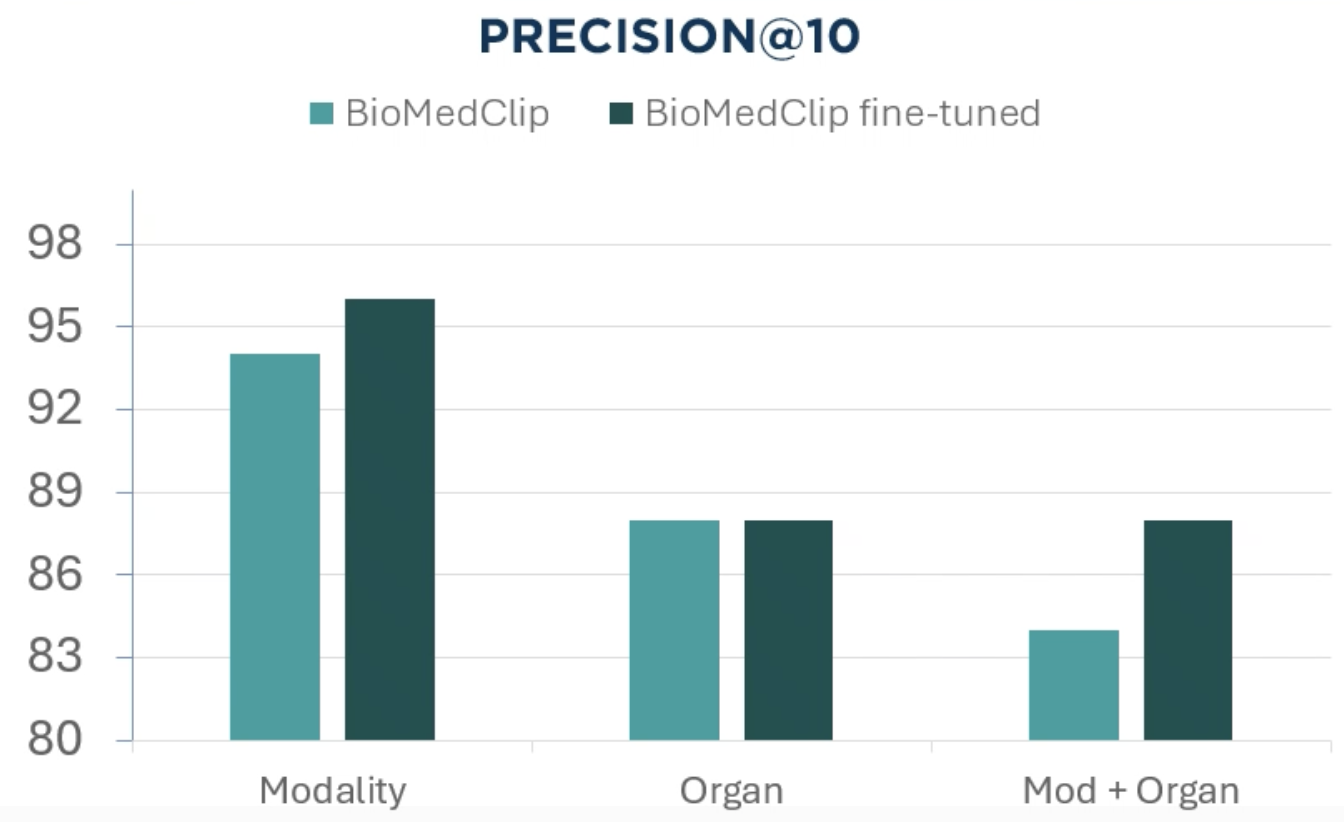
\includegraphics[width=\textwidth]{assets/biomedclipPrec.png}
  \captionsetup{justification=centering, singlelinecheck=false}
  \captionof{figure}{BioMedCLIP : Precision@k}
\end{minipage}
\hfill
\begin{minipage}[t]{0.48\textwidth}
  \centering
  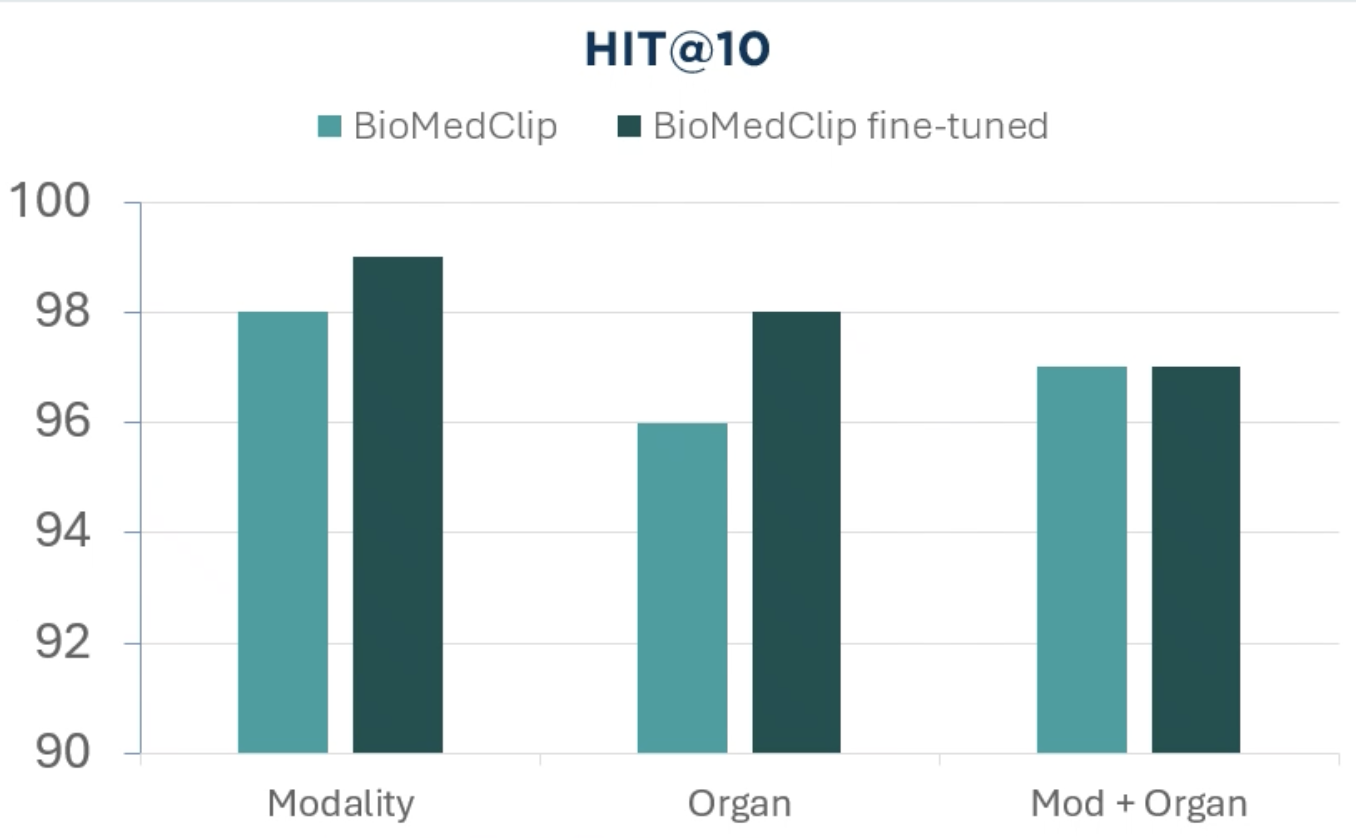
\includegraphics[width=\textwidth]{assets/biomedclipHIT.png}
  \captionsetup{justification=centering, singlelinecheck=false}
  \captionof{figure}{BioMedCLIP : Hit@k}
\end{minipage}

\vspace{0.3cm}
\noindent{\small\textbf{Interprétation.}
BioMedCLIP capte mieux le \textbf{sens clinique} grâce à son alignement image-texte
fine-tuné sur ROCOv2. Ses scores combinant modalité et organe sont supérieurs à DINOv2,
validant son usage pour la recherche sémantique.}

\vspace{0.7cm}

\subsection{Tests unitaires}

\vspace{0.2cm}
Une stratégie de tests \textbf{unitaires} et \textbf{d'intégration} a été mise en place
pour garantir la fiabilité du backend et la stabilité du pipeline de recherche.

\vspace{0.2cm}
\begin{sq}
  \item \textbf{Backend :} tests \texttt{pytest} couvrant les neuf endpoints REST,
        validation des entrées, formats de réponse, gestion des erreurs.
  \item \textbf{Pipeline CBIR :} tests sur les embedders, le chargement des index
        \textbf{FAISS} et la cohérence des résultats de recherche.
  \item \textbf{Intégration :} scénarios bout-en-bout simulant une requête utilisateur
        depuis l'upload d'image jusqu'au retour des résultats.
\end{sq}

\vspace{0.7cm}

\subsection{Performance technique}

\vspace{0.2cm}
Au-delà de la pertinence des résultats, le système a été évalué sur ses
\textbf{performances en production}.

\vspace{0.2cm}
\begin{sq}
  \item \textbf{Temps de réponse :} recherche vectorielle exécutée en
        \textbf{quelques centaines de millisecondes} sur l'index de 60\,000 vecteurs.
  \item \textbf{Empreinte mémoire :} chargement \textit{lazy} des modèles et de l'index
        pour limiter la consommation au démarrage.
  \item \textbf{Scalabilité :} architecture \textit{stateless} permettant de déployer
        plusieurs instances backend derrière Nginx pour absorber la charge.
\end{sq}

\vspace{0.7cm}

\subsection{Limites observées et synthèse}

\vspace{0.2cm}
\begin{sq}
  \item \textbf{Modalités rares :} les modalités sous-représentées dans ROCOv2 obtiennent des scores plus faibles que les modalités majoritaires.
  \item \textbf{Captions ambiguës :} la recherche textuelle est sensible à la qualité et à la précision de la description fournie.
  \item \textbf{Dépendance au dataset :} les performances reflètent le périmètre de ROCOv2 et ne préjugent pas du comportement sur d'autres corpus médicaux.
\end{sq}

\vspace{0.3cm}
\noindent\textbf{Synthèse.}
Malgré ces limites, les résultats valident la pertinence de \textbf{MEDISCAN AI} :
les deux moteurs sont \textbf{complémentaires} (DINOv2 pour la proximité visuelle,
BioMedCLIP pour le sens clinique), les tests garantissent la fiabilité du système
et les performances permettent un usage fluide en production.

% =========================================================
% CHAPITRE 8 — Difficultés rencontrées
% =========================================================
\NewMajorPart
\section{Difficultés rencontrées}

\vspace{0.2cm}
Cette section revient sur les principales difficultés rencontrées au cours du projet.

\vspace{0.5cm}

\subsection{Fine-tuning et choix des modèles}

\vspace{0.15cm}
Plusieurs candidats existaient pour la partie sémantique (BioMedCLIP, PubMedCLIP, MedCLIP).

\vspace{0.15cm}
\begin{sq}
  \item \textbf{Choix du modèle :} sélection de \textbf{BioMedCLIP} pour son alignement image-texte biomédical.
  \item \textbf{Fine-tuning :} adaptation à \textbf{ROCOv2} avec plusieurs itérations d'hyperparamètres.
  \item \textbf{Ressources GPU limitées :} entraînement sur les GPU \textbf{Kaggle}, avec des quotas contraints.
\end{sq}

\vspace{0.5cm}

\subsection{Manipulation d'un dataset volumineux}

\vspace{0.15cm}
Les \textbf{60\,000 images} de ROCOv2 ont soulevé plusieurs défis de volumétrie.

\vspace{0.15cm}
\begin{sq}
  \item \textbf{Stockage et bande passante :} dépendance à \textbf{Hugging Face}, téléchargements non négligeables.
  \item \textbf{Génération des embeddings :} opération longue et coûteuse en mémoire sur les deux modèles.
  \item \textbf{Manque de ressources cloud :} pas de cluster GPU dédié, contraintes mémoire sur le VPS.
\end{sq}

\vspace{0.5cm}

\subsection{Absence de benchmark de référence en CBIR médical}

\vspace{0.15cm}
Aucun \textbf{benchmark standardisé} n'existe pour évaluer un système CBIR médical multimodal.

\vspace{0.15cm}
\begin{sq}
  \item \textbf{Méthodologie ad hoc :} démarche d'évaluation construite à partir des métadonnées.
  \item \textbf{Annotations expertes :} mobilisation de \textbf{doctorants en imagerie médicale} pour la vérité terrain.
  \item \textbf{Comparabilité :} difficulté à confronter les résultats à d'autres systèmes.
\end{sq}

% =========================================================
% CHAPITRE 9 — Bilan et retour d'expérience
% =========================================================
\NewMajorPart
\section{Bilan et retour d'expérience}

Cette section dresse un bilan du projet, à la fois sur les acquis techniques
et sur l'expérience humaine vécue par l'équipe au cours du semestre.

\vspace{0.15cm}

\subsection{Réussites techniques}

Le projet a abouti à une plateforme fonctionnelle, complète et déployée en production,
accessible publiquement à l'adresse \texttt{mediscan-ai.site}.
\begin{sq}
  \item \textbf{Multimodalité :} intégration réussie de la recherche visuelle, sémantique et textuelle dans une seule interface cohérente.
  \item \textbf{Mise en production :} déploiement complet sur VPS avec \textbf{Nginx}, \textbf{SSL} et services systemd pour garantir la stabilité du service.
  \item \textbf{Fine-tuning :} adaptation effective de \textbf{BioMedCLIP} sur ROCOv2, avec des résultats validés par les doctorants en imagerie médicale.
\end{sq}

\vspace{0.15cm}

\subsection{Apports méthodologiques}

Le projet a permis de structurer une démarche complète d'ingénierie logicielle
appliquée à un cas concret d'intelligence artificielle.
\begin{sq}
  \item \textbf{Cycle incrémental :} découpage en quatre livrables successifs, du cœur CBIR au déploiement final.
  \item \textbf{Évaluation rigoureuse :} construction d'une méthodologie d'évaluation appuyée sur des annotations expertes et plus de 9\,000 requêtes.
  \item \textbf{Versionnement collaboratif :} usage quotidien de \textbf{Git} avec branches de fonctionnalités, revues croisées et historique propre.
\end{sq}

\vspace{0.15cm}

\subsection{Apports humains et travail d'équipe}

Au-delà des aspects techniques, le projet a constitué une véritable expérience
de collaboration et d'apprentissage collectif.
\begin{sq}
  \item \textbf{Spécialisation progressive :} chaque membre a développé une expertise reconnue (IA, frontend, backend, tests).
  \item \textbf{Coordination :} points de synchronisation réguliers sur \textbf{Discord} pour partager les blocages et avancées.
  \item \textbf{Polyvalence :} contribution croisée de chaque membre à plusieurs composants du système, renforçant la cohésion d'équipe.
\end{sq}

% =========================================================
% CHAPITRE 10 — Impact agentic AI
% =========================================================
\NewMajorPart
\section{Impact agentic AI}

Cette section revient sur l'usage des IA agentiques dans la réalisation du projet
et sur leur apport à la productivité de l'équipe.

\vspace{0.15cm}

\subsection{État actuel des IA agentiques}

Les modèles d'IA dits \textbf{agentiques} ont connu une évolution rapide en 2024-2025,
passant de simples assistants conversationnels à de véritables collaborateurs capables
d'agir sur du code, des fichiers et des outils.
\begin{sq}
  \item \textbf{Claude (Anthropic)} et \textbf{Codex (OpenAI)} dominent les usages développeurs avec leurs capacités d'écriture, de relecture et de refactorisation de code.
  \item Les agents savent désormais \textbf{exécuter des commandes}, lire des logs, modifier plusieurs fichiers et raisonner sur un projet entier.
\end{sq}

\vspace{0.15cm}

\subsection{Utilisation dans le projet}

L'équipe a intégré ces outils à différentes étapes du développement, de la conception
à la rédaction du rapport, à travers des prompts ciblés.
\begin{sq}
  \item \textbf{Génération de code :} \textit{« Écris un endpoint FastAPI qui retourne les k plus proches voisins via FAISS à partir d'une image uploadée. »}
  \item \textbf{Debug et refactorisation :} \textit{« Pourquoi ce test pytest échoue ? Propose un correctif. »}
  \item \textbf{Rédaction et structuration :} \textit{« Rédige la section Évaluation en t'appuyant sur les graphiques DINOv2 et BioMedCLIP. »}
\end{sq}

\vspace{0.15cm}

\subsection{Apports et limites}

L'usage des IA agentiques a transformé la manière de travailler, sans pour autant
remplacer le jugement humain.
\begin{sq}
  \item \textbf{Avantages :} accélération du développement, exploration rapide de pistes techniques, qualité de code améliorée et gain de temps sur les tâches répétitives.
  \item \textbf{Limites :} nécessité de relire systématiquement les sorties, risques d'hallucinations sur des contextes pointus, dépendance à un service externe.
  \item \textbf{Posture adoptée :} l'IA reste un assistant ; chaque proposition est validée, testée et adaptée par l'équipe avant intégration.
\end{sq}

% =========================================================
% CHAPITRE 11 — Perspectives
% =========================================================
\NewMajorPart
\section{Perspectives}

\vspace{0.2cm}
Plusieurs pistes d'évolution se dessinent pour prolonger et enrichir \textbf{MEDISCAN AI}.

\vspace{0.5cm}

\subsection{Évolutions fonctionnelles}

\vspace{0.15cm}
La plateforme peut s'enrichir de nouvelles capacités côté utilisateur.

\vspace{0.15cm}
\begin{sq}
  \item \textbf{Support du format DICOM :} ingestion native des images médicales au format standard hospitalier.
  \item \textbf{Recherche par filtres avancés :} combinaison de critères cliniques (modalité, organe, pathologie).
  \item \textbf{Export enrichi :} génération de rapports PDF combinant images, scores et synthèse IA.
\end{sq}

\vspace{0.5cm}

\subsection{Évolutions techniques}

\vspace{0.15cm}
L'infrastructure et les modèles peuvent être renforcés pour passer à l'échelle.

\vspace{0.15cm}
\begin{sq}
  \item \textbf{Pipeline CI/CD :} automatisation des tests, du build et du déploiement à chaque commit.
  \item \textbf{Index FAISS optimisé :} passage d'un index \textbf{FlatIP} à un index \textbf{IVF} ou \textbf{HNSW} pour des volumes supérieurs.
  \item \textbf{Fine-tuning continu :} ré-entraînement régulier sur de nouvelles données pour améliorer la pertinence.
\end{sq}

\vspace{0.5cm}

\subsection{Vers la recherche et l'industrie}

\vspace{0.15cm}
\textbf{MEDISCAN AI} ouvre des perspectives concrètes d'usage au-delà du cadre académique.

\vspace{0.15cm}
\begin{sq}
  \item \textbf{Intégration aux systèmes PACS :} brancher le moteur multimodal sur les bases hospitalières existantes.
  \item \textbf{Partenariats cliniques :} collaboration avec des établissements pour valider l'usage en conditions réelles.
  \item \textbf{Publications et benchmarks :} contribuer à combler le manque de standards d'évaluation en CBIR médical.
\end{sq}

% =========================================================
% RÉFÉRENCES BIBLIOGRAPHIQUES
% =========================================================
\NewMajorPart
\section*{Références bibliographiques}
\addcontentsline{toc}{section}{Références bibliographiques}

\begin{num}
  \item M.~Caron \textit{et al.}, ``Emerging Properties in Self-Supervised Vision
        Transformers,'' \textit{ICCV}, 2021.
  \item S.~Zhang \textit{et al.}, ``BioMedCLIP: a multimodal biomedical foundation
        model,'' \textit{arXiv:2303.00915}, 2023.
  \item J.~Johnson, M.~Douze, H.~Jégou, ``Billion-scale similarity search with GPUs,''
        \textit{IEEE Transactions on Big Data}, 2019.
  \item FastAPI Documentation. \url{https://fastapi.tiangolo.com}
  \item React Documentation. \url{https://react.dev}
\end{num}

% =========================================================
% ANNEXES
% =========================================================
\NewMajorPart
\appendix

\section{Documentation API REST}

Les neuf endpoints de l'API sont exposés sous la base \texttt{/api/v1}.

\vspace{0.3cm}
\begin{table}[H]
\centering
\begin{tabularx}{\textwidth}{@{}llX@{}}
\toprule
\textbf{Méthode} & \textbf{Endpoint} & \textbf{Description} \\
\midrule
POST & \texttt{/search/visual}    & Recherche visuelle par image (DINOv2). \\
POST & \texttt{/search/semantic}  & Recherche sémantique par image (BioMedCLIP). \\
POST & \texttt{/search/text}      & Recherche par description textuelle (BioMedCLIP). \\
POST & \texttt{/search/multisel}  & Relance depuis une sélection d'images (centroïde). \\
GET  & \texttt{/synthesis}        & Génère la synthèse IA pour un ensemble de résultats. \\
GET  & \texttt{/export/json}      & Export des résultats au format JSON. \\
GET  & \texttt{/export/csv}       & Export des résultats au format CSV. \\
GET  & \texttt{/export/pdf}       & Export des résultats au format PDF. \\
GET  & \texttt{/health}           & Vérification de l'état du service. \\
\bottomrule
\end{tabularx}
\caption{Endpoints REST exposés par l'API MEDISCAN AI}
\label{tab:api-rest}
\end{table}

\section{Extraits de code et utilisation de l'IA}

\IntroPartie{Cette annexe présente les extraits de code les plus significatifs
du projet MEDISCAN AI, illustrant les choix d'implémentation des composants
centraux du système : les encodeurs d'images, le moteur de recherche FAISS,
et l'utilisation de l'intelligence artificielle au cours du développement.}

% =========================================================
% PACKAGES NÉCESSAIRES (à ajouter dans le préambule)
% \usepackage{listings}
% \usepackage{xcolor}
% =========================================================

% Style listings
\lstdefinestyle{mediscan}{
  backgroundcolor=\color{gray!7},
  basicstyle=\ttfamily\footnotesize,
  keywordstyle=\color{teal}\bfseries,
  commentstyle=\color{gray}\itshape,
  stringstyle=\color{orange!80!black},
  breaklines=true,
  frame=single,
  rulecolor=\color{gray!30},
  numbers=left,
  numberstyle=\tiny\color{gray},
  numbersep=8pt,
  showstringspaces=false,
  tabsize=4,
  language=Python,
}

% =========================================================
\subsection{Encodeur BioMedCLIP}
% =========================================================

\noindent L'encodeur BioMedCLIP est le composant central du mode Analyse
Interprétative. Il encode les images et les requêtes textuelles dans un
espace vectoriel commun de dimension 512, permettant la recherche sémantique
multimodale. Le modèle utilisé est une version fine-tunée sur ROCOv2,
hébergée sur HuggingFace sous l'identifiant
\texttt{Ozantsk/biomedclip-rocov2-finetuned}.

\begin{lstlisting}[style=mediscan, caption={Implémentation de l'encodeur BioMedCLIP (src/mediscan/embedders/biomedclip.py)}]
class BioMedCLIPEmbedder(Embedder):
    """
    BioMedCLIP image and text embedder for semantic medical search.
    The image and text encoders share the same vector space, allowing
    text prompts and medical images to query the same semantic FAISS index.
    """
    name = "biomedclip"
    dim = 512

    def __init__(
        self,
        model_name: str = "hf-hub:Ozantsk/biomedclip-rocov2-finetuned",
    ) -> None:
        configure_torch_cpu_threads()
        self._device = torch.device("cpu")
        self._model, _, self._preprocess = open_clip.create_model_and_transforms(
            model_name
        )
        self._model.to(self._device)
        self._model.eval()
        self._tokenizer = open_clip.get_tokenizer(model_name)

    def encode_pil(self, image: PILImage.Image) -> np.ndarray:
        """Encode a PIL image into the normalized semantic vector space."""
        rgb_image = image.convert("RGB")
        input_tensor = self._preprocess(rgb_image).unsqueeze(0).to(self._device)
        with torch.no_grad():
            features = self._model.encode_image(input_tensor)
        return normalize_embedding(features.squeeze(0).cpu().numpy(), self.dim)

    def encode_text(self, text: str) -> np.ndarray:
        """Encode a text query into the same normalized space as image embeddings."""
        tokens = self._tokenizer([text]).to(self._device)
        with torch.no_grad():
            features = self._model.encode_text(tokens)
        return normalize_embedding(features.squeeze(0).float().cpu().numpy(), self.dim)
\end{lstlisting}

% =========================================================
\subsection{Encodeur DINOv2}
% =========================================================

\noindent L'encodeur DINOv2 est le composant central du mode Analyse Visuelle.
Il produit des vecteurs de dimension 768 capturant la structure anatomique et
visuelle des images médicales, sans avoir été entraîné sur des données médicales.
Le \textit{pooler output} est utilisé en priorité ; le token CLS est utilisé
comme alternative si le modèle ne l'expose pas.

\begin{lstlisting}[style=mediscan, caption={Implémentation de l'encodeur DINOv2 (src/mediscan/embedders/dinov2\_base.py)}]
class DINOv2BaseEmbedder(Embedder):
    """
    DINOv2 base image embedder for visual similarity search.
    Compares image content directly without text supervision at query time.
    """
    name = "dinov2_base"
    dim = 768

    def __init__(self, model_name: str = "facebook/dinov2-base") -> None:
        configure_torch_cpu_threads()
        self._device = torch.device("cpu")
        self._processor = AutoImageProcessor.from_pretrained(
            model_name, use_fast=True
        )
        self._model = AutoModel.from_pretrained(model_name)
        self._model.to(self._device)
        self._model.eval()

    def encode_pil(self, image: PILImage.Image) -> np.ndarray:
        """Encode a PIL image into a normalized visual embedding vector."""
        rgb_image = image.convert("RGB")
        inputs = self._processor(images=rgb_image, return_tensors="pt")
        pixel_values = inputs["pixel_values"].to(self._device)

        with torch.no_grad():
            outputs = self._model(pixel_values=pixel_values)

        # Pooler output preferred; CLS token used as fallback
        if getattr(outputs, "pooler_output", None) is not None:
            features = outputs.pooler_output
        else:
            features = outputs.last_hidden_state[:, 0]

        return normalize_embedding(features.squeeze(0).cpu().numpy(), self.dim)
\end{lstlisting}

% =========================================================
\subsection{Moteur de recherche FAISS}
% =========================================================

\noindent Le moteur de recherche centralise le chargement des ressources,
l'encodage des requêtes et la recherche dans l'index FAISS. Trois types de
requêtes sont supportés : par image uploadée, par identifiant d'image déjà
indexée, et par texte médical.

\begin{lstlisting}[style=mediscan, caption={Recherche par image uploadée (src/mediscan/search.py)}]
def query(
    *,
    resources: SearchResources,
    image: str | Path,
    k: int,
    exclude_self: bool = False,
) -> list[dict[str, Any]]:
    """Encode a query image and search the matching FAISS index."""
    _validate_k(k)
    query_image = resolve_path(image)

    with Image.open(query_image) as pil_image:
        query_vector = (
            resources.embedder.encode_pil(pil_image)
            .reshape(1, -1)
            .astype(np.float32)
        )
    faiss.normalize_L2(query_vector)

    search_k = compute_search_k(k, resources.index.ntotal, exclude_self=exclude_self)
    scores, indices = resources.index.search(query_vector, search_k)

    excluded_ids = {query_image.stem} if exclude_self else set()
    excluded_paths = {str(query_image.resolve())} if exclude_self else set()

    return collect_ranked_results(
        rows=resources.rows,
        scores=scores[0],
        indices=indices[0],
        k=k,
        excluded_image_ids=excluded_ids,
        excluded_paths=excluded_paths,
    )
\end{lstlisting}

\begin{lstlisting}[style=mediscan, caption={Recherche par texte médical (src/mediscan/search.py)}]
def query_text(
    *,
    resources: SearchResources,
    text: str,
    k: int,
) -> list[dict[str, Any]]:
    """Encode a text prompt and search the semantic FAISS index."""
    _validate_k(k)
    if not hasattr(resources.embedder, "encode_text"):
        raise ValueError(
            "Embedder does not support encode_text(). "
            "Use mode='semantic' (BioMedCLIP) for text queries."
        )

    query_vector = (
        resources.embedder.encode_text(text.strip())
        .reshape(1, -1)
        .astype(np.float32)
    )
    faiss.normalize_L2(query_vector)

    search_k = compute_search_k(k, resources.index.ntotal)
    scores, indices = resources.index.search(query_vector, search_k)

    return collect_ranked_results(
        rows=resources.rows,
        scores=scores[0],
        indices=indices[0],
        k=k,
    )
\end{lstlisting}

% =========================================================
\subsection{Utilisation de l'intelligence artificielle}
% =========================================================

\noindent Au cours du développement de MEDISCAN AI, des outils d'intelligence
artificielle générative ont été utilisés à plusieurs étapes du projet :
génération de code, débogage, rédaction de documentation et aide à la
conception. Les exemples ci-dessous illustrent quelques-uns des prompts
rédigés par l'équipe.

\vspace{0.4cm}

\begin{promptbox}
Implémente une classe Python \texttt{BioMedCLIPEmbedder} qui charge le modèle
\texttt{hf-hub:Ozantsk/biomedclip-rocov2-finetuned} via \texttt{open\_clip},
expose une méthode \texttt{encode\_pil} pour encoder une image PIL, et une
méthode \texttt{encode\_text} pour encoder une requête textuelle. Les deux
méthodes doivent retourner un vecteur numpy normalisé L2 de dimension 512.
\end{promptbox}

\textit{Ce prompt a servi de base à l'implémentation de l'encodeur BioMedCLIP,
ensuite adaptée et intégrée au pipeline MEDISCAN AI.}

\vspace{0.5cm}

\begin{promptbox}
Comment implémenter une recherche de voisins les plus proches avec FAISS
\texttt{IndexFlatIP} sur des embeddings normalisés L2 de dimension 768 ?
La fonction doit accepter un vecteur requête numpy, retourner les $k$ résultats
les plus similaires avec leurs scores, et exclure l'image requête elle-même
des résultats si elle est déjà indexée.
\end{promptbox}

\textit{Ce prompt a guidé l'implémentation du moteur de recherche vectorielle,
notamment la gestion de l'exclusion de la requête et du paramètre \texttt{search\_k}.}

\vspace{0.5cm}

\begin{promptbox}
Écris un script Python d'évaluation qui mesure la Precision@k d'un index FAISS
sur trois critères : même modalité (TM), même organe (TA), et même modalité et
organe (TMO), à partir de fichiers CSV de ground truth. Le script doit accepter
les arguments \texttt{--mode}, \texttt{--k}, \texttt{--n-queries} et
\texttt{--seed}, et afficher la progression toutes les 500 requêtes.
\end{promptbox}

\textit{Ce prompt a fourni la structure du script \texttt{evaluate\_strict.py},
qui a ensuite été enrichi avec la gestion du pool de candidats et l'export CSV.}

\vspace{0.5cm}

\begin{promptbox}
Prouve mathématiquement qu'il est impossible de reconstruire une image médicale
depuis son embedding DINOv2 de dimension 768. Calcule le ratio de compression
pour une image de $682 \times 748$ pixels et explique pourquoi la perte
d'information est irréversible.
\end{promptbox}

\textit{Ce prompt a permis de formaliser l'argument de confidentialité des données
présenté dans la gouvernance du système et dans la politique de confidentialité
de l'application.}

\section{Résultats de tests détaillés}

\IntroPartie{Les évaluations ont été conduites sur un sous-ensemble de 200 images
requêtes pour les modes visuel et sémantique, et sur 100 images pour la recherche
par texte, échantillonnées aléatoirement avec la graine 42 depuis le ground truth
disponible. Trois critères de pertinence ont été définis : TM (même modalité),
TA (même organe), et TMO (même modalité et même organe). La métrique principale
est la \textbf{Precision@10}.}

\subsection{Mode Analyse Visuelle (DINOv2)}

Sur 200 requêtes évaluées avec $k=10$, le mode Analyse Visuelle obtient une
Precision@10 de \textbf{93,25\%} sur le critère TM, \textbf{37,40\%} sur le
critère TA, et \textbf{36,00\%} sur le critère TMO. Ces résultats montrent que
DINOv2 est particulièrement efficace pour retrouver des images de même modalité
d'imagerie, ce qui est cohérent avec sa nature de modèle visuel généraliste
capturant la structure globale des images. En revanche, la précision sur l'organe
seul ou la combinaison modalité-organe est plus faible, ce qui s'explique par le
fait que DINOv2 n'a jamais été entraîné sur des données médicales annotées.

\begin{center}
\begin{tabularx}{0.7\textwidth}{@{}lX@{}}
\toprule
\textbf{Critère} & \textbf{Precision@10} \\
\midrule
TM — Même modalité          & 93,25\% \\
TA — Même organe            & 37,40\% \\
TMO — Modalité + organe     & 36,00\% \\
\bottomrule
\end{tabularx}
\end{center}

\subsection{Mode Analyse Interprétative (BioMedCLIP)}

Sur les mêmes 200 requêtes avec $k=10$, le mode Analyse Interprétative obtient
une Precision@10 de \textbf{93,45\%} sur TM, \textbf{46,80\%} sur TA, et
\textbf{44,10\%} sur TMO. BioMedCLIP surpasse DINOv2 sur les critères TA et TMO,
avec un gain de $+9,40$ points sur l'organe et $+8,10$ points sur la combinaison
modalité-organe. Ce résultat confirme l'apport du fine-tuning sur ROCOv2 et de
l'alignement image-texte médical pour capturer la sémantique clinique des images
au-delà de leur apparence visuelle.

\begin{center}
\begin{tabularx}{0.7\textwidth}{@{}lX@{}}
\toprule
\textbf{Critère} & \textbf{Precision@10} \\
\midrule
TM — Même modalité          & 93,45\% \\
TA — Même organe            & 46,80\% \\
TMO — Modalité + organe     & 44,10\% \\
\bottomrule
\end{tabularx}
\end{center}

\subsection{Mode Recherche par Texte (BioMedCLIP)}

L'évaluation de la recherche par texte a été conduite sur 100 images en deux
modes : \textit{caption} (légende complète utilisée comme requête) et
\textit{keyword} (mots-clés extraits de la légende).

En mode \textbf{caption}, le système atteint une Precision@10 de
\textbf{98,10\%}, un Top-1 hit de \textbf{17,00\%} et un Recall@10 de
\textbf{49,00\%}. La Precision@10 très élevée indique que les résultats retournés
sont quasi-systématiquement pertinents. Le Top-1 hit de 17\% signifie que dans
17\% des cas, l'image source elle-même est classée en première position, ce qui
est remarquable compte tenu de la taille de la base.

En mode \textbf{keyword}, la Precision@10 reste solide à \textbf{94,50\%}, mais
le Top-1 hit tombe à \textbf{0,00\%} et le Recall@10 à \textbf{7,00\%}. Ce
résultat est attendu : une requête réduite à quelques mots-clés est une
représentation moins précise de l'image source, ce qui rend le rappel de l'image
exacte beaucoup plus difficile. Néanmoins, la haute précision montre que même
avec une requête partielle, le système retrouve des images cliniquement
pertinentes.

\begin{center}
\begin{tabularx}{0.85\textwidth}{@{}lXXX@{}}
\toprule
\textbf{Mode} & \textbf{Precision@10} & \textbf{Top-1 hit} & \textbf{Recall@10} \\
\midrule
Caption  & 98,10\% & 17,00\% & 49,00\% \\
Keyword  & 94,50\% &  0,00\% &  7,00\% \\
\bottomrule
\end{tabularx}
\end{center}

\newpage
\section{Glossaire}
\begin{description}[leftmargin=7em, style=sameline]
  \item[BioMedCLIP] Modèle multimodal pré-entraîné sur des données biomédicales, alignant
                    images et textes dans un espace vectoriel commun de dimension 512.
  \item[CBIR]       \textit{Content-Based Image Retrieval} --- recherche d'images
                    par le contenu visuel ou sémantique, sans recours à des métadonnées
                    textuelles manuelles.
  \item[Centroïde]  Vecteur moyen de plusieurs embeddings, utilisé pour la relance
                    multi-sélection afin de représenter la tendance commune d'un groupe.
  \item[CUI]        \textit{Concept Unique Identifier} --- identifiant unique d'un concept
                    dans la nomenclature médicale UMLS.
  \item[DINOv2]     Modèle de vision auto-supervisé développé par Meta AI, utilisé pour
                    extraire des représentations visuelles de dimension 768.
  \item[Embedding]  Représentation vectorielle d'une image ou d'un texte dans un espace
                    de grande dimension, calculée par un réseau de neurones.
  \item[FAISS]      \textit{Facebook AI Similarity Search} --- bibliothèque de recherche
                    de voisins les plus proches dans des espaces vectoriels de grande dimension.
  \item[FastAPI]    Framework Python asynchrone pour la création d'API REST, utilisé comme
                    couche applicative backend du système.
  \item[Fine-tuning] Adaptation d'un modèle pré-entraîné à un domaine spécifique par un
                    entraînement complémentaire sur des données ciblées.
  \item[Groq]       Service d'inférence LLM rapide, utilisé pour la génération de la
                    synthèse assistée.
  \item[LLM]        \textit{Large Language Model} --- modèle de langage de grande taille,
                    utilisé ici pour générer une synthèse exploratoire à partir des résultats.
  \item[MongoDB]    Base de données orientée documents, utilisée pour l'enrichissement
                    optionnel des métadonnées associées aux résultats de recherche.
  \item[React]      Bibliothèque JavaScript pour la construction d'interfaces utilisateur,
                    utilisée pour le frontend du système.
  \item[ROCOv2]     \textit{Radiology Objects in Context v2} --- dataset public d'images
                    médicales annotées avec des captions et des concepts UMLS (CUI).
  \item[Top-k]      Les $k$ résultats les plus similaires à une requête, retournés par
                    ordre décroissant de similarité.
  \item[UMLS]       \textit{Unified Medical Language System} --- système de terminologie
                    médicale unifié, référence pour les concepts cliniques.
  \item[Vite]       Outil de build et de développement frontend rapide, utilisé pour
                    compiler et servir l'application React.
\end{description}

% =========================================================
% INDEX
% =========================================================
\NewMajorPart
\printindex

% =========================================================
\end{document}
% =========================================================